\usetikzlibrary{calc}
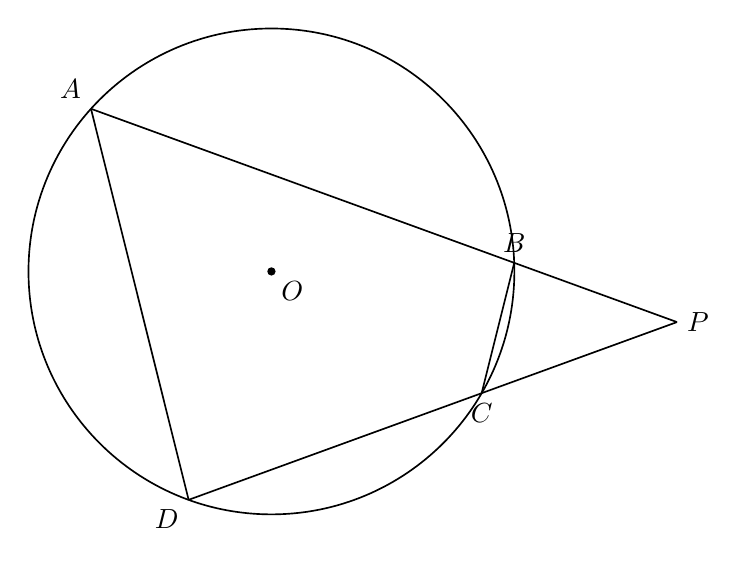
\begin{tikzpicture}[x=1cm,y=1cm,line width=.6pt,font=\normalsize]
\coordinate (P) at (0.0,0.0);
\coordinate (B) at (-2.0673,0.7524);
\coordinate (A) at (-7.4424,2.7088);
\coordinate (C) at (-2.4808,-0.9029);
\coordinate (D) at (-6.202,-2.2573);
\coordinate (O) at (-5.1506,0.6432);
\draw (O) circle[radius=3.0852cm];
\draw (P)--(A);
\draw (P)--(D);
\draw (A)--(D);
\draw (B)--(C);
\fill (O) circle(1.5pt);
\node[right] at (P) {$P$};
\node[above left] at (A) {$A$};
\node[above] at (B) {$B$};
\node[below] at (C) {$C$};
\node[below left] at (D) {$D$};
\node[below right] at (O) {$O$};
\end{tikzpicture}
